\documentclass{article}
\usepackage[utf8]{inputenc}
\usepackage[top= 0.3in]{geometry}
\usepackage{cite}

\title{Aprendizagem de Máquina}
\author{Iasmym Lorany Mendes de França}
\date{05 de Novembro de 2019}

\usepackage{natbib}
\usepackage{graphicx}

\begin{document}

\maketitle

\section{Introdução}
\hspace{0.5in}Aprendizagem de Máquina (em  inglês, machine learning) é o campo da computação, advindo da inteligência artificial, que estuda o treinamento de máquinas para aprenderem com análise de dados e identificação de padrões, muitas vezes com nenhuma intervenção humana.

\hspace{0.5in}\textit{"Machine learning: field of study that gives computers the ability to learn without being explicitly programmed”}\cite{arthursamuel}

\begin{figure}[h!]
\centering
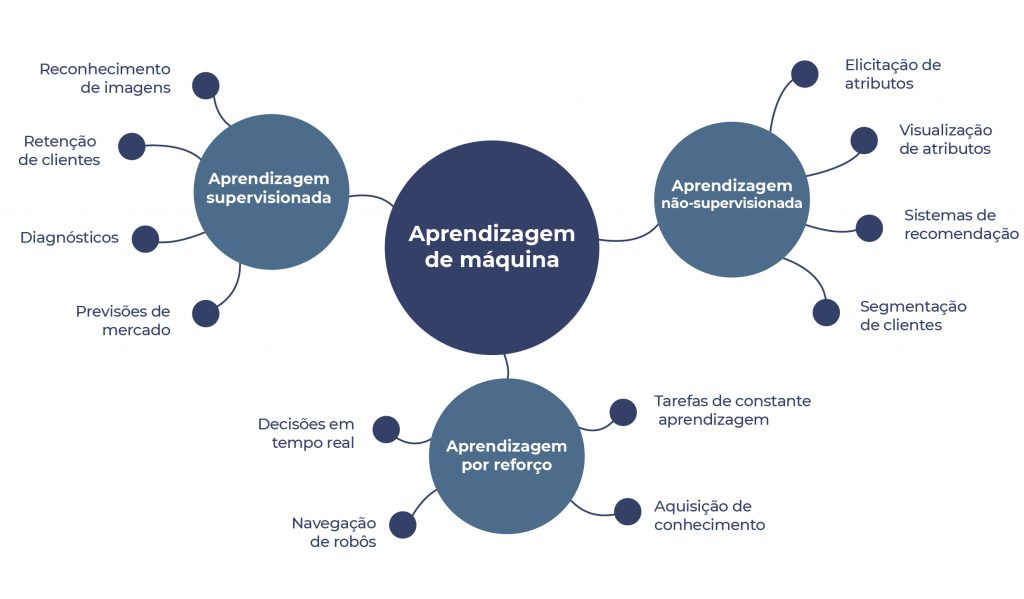
\includegraphics[scale=0.5]{aprendizagem.jpg}
\caption{Principais sub divisões e aplicabilidade da aprendizagem de máquina\hspace{0.02in}\cite{isitics}}
\label{fig:aprendizagem}
\end{figure}

\section{Relevância}
\hspace{0.5in}Vivemos na era da "big data", nunca houve uma produção de dados tão grande como últimos 20 anos e a aprendizagem de máquina está diretamente ligada a como aproveitamos tais dados. Um exemplo simples e relevante de sua aplicação no dia a dia são sites como Netflix e Spotify, que baseiam-se no histórico de acesso do usuário para recomendar novos filmes e músicas. Desde aplicações simples a mais complexas, como diagnósticos médicos \cite{medico}, a aprendizagem de máquina promete estar cada dia mais presente em nossas vidas com rápida evolução da tecnolgia.

\hspace{0.5in}Alguns outros exemplos de sua aplicação \cite{aplicacao}:

 \begin{itemize}
     \item Deteccção de Fraudes
     \item Mecanismos de Busca
     \item Bots de Serviço ao Cliente
     \item Veículos Autônomos
 \end{itemize}

\section{Relação com outras disciplinas}
\hspace{0.5in}A disciplina de Aprendizagem de Máquina possui as seguintes disciplinas como pré-requisitos:

\begin{itemize}
    \item IF684 - Sistemas Inteligentes: o entendimento do funcionamento de sistemas inteligentes é essencial, visto que tal disciplina tem ligação direta com inteligência artifical, do qual originou-se a aprendizagem de máquina, e lida com resoluções em big data, importante fator no estudo da análise de dados.
    
    \item ET586 - Estatística e Probabilidades para Computação: sendo um dos fatores mais importantes da aprendizagem de máquina, estatística e probabilidade estão relacionadas com a análise da frequência de eventos \cite{probs}, que tendem a serem aplicados em diversos campos de estudo e aplicações da aprendizagem de máquina.
    
\end{itemize}

\bibliographystyle{plain}
\bibliography{ilmf}
\end{document}